\documentclass[11pt, a4paper]{article}

\usepackage[utf8]{inputenc}
\usepackage[T1]{fontenc}
\usepackage{kotex}
\usepackage{graphicx}
\usepackage{booktabs}
\usepackage{caption}
\usepackage{geometry}
\usepackage{hyperref}
\usepackage{float}
\usepackage{xcolor}
\usepackage{fancyhdr}
\usepackage{multirow}
\usepackage{array}
\usepackage{tocloft}

\geometry{margin=2.5cm}
\pagestyle{fancy}
\fancyhf{}
\rhead{EmpathyAI Project Report}
\cfoot{\thepage}

\definecolor{primary}{HTML}{2C3E50}
\definecolor{accent}{HTML}{27AE60}

\captionsetup{format=plain, labelfont=bf, font=small, labelsep=newline, justification=raggedright, singlelinecheck=false}

\begin{document}

% ============================================
% 표지
% ============================================
\begin{titlepage}
    \centering
    \vspace*{2cm}
    {\Huge\bfseries\color{primary} EmpathyAI\par}
    \vspace{1cm}
    {\LARGE Project Final Report\par}
    \vspace{1.5cm}
    {\large LLM Fine-tuning for Empathy Level Classification\par}
    \vspace{0.5cm}
    {\large OPELA Dataset based GPT-4.1 Nano \& DeepSeek 7B Optimization\par}
    \vspace{2cm}
    
    \begin{tabular}{|l|r|}
    \hline
    Base Model Accuracy: & 15.70\% \\
    \hline
    GPT Fine-tuned Accuracy: & 33.49\% \\
    \hline
    \textbf{DeepSeek QLoRA Accuracy:} & \textbf{\textcolor{accent}{49.19\%}} \\
    \hline
    Best Improvement: & \textcolor{accent}{+33.49\%p} \\
    \hline
    \end{tabular}
    
    \vspace{2cm}
    {\large 2025-12-17\par}
    \vspace{1cm}
    {\large Based on Smilegate AI \& Seoul National University Research Data\par}
\end{titlepage}

% ============================================
% 목차
% ============================================
\tableofcontents
\newpage

% ============================================
% 1. Introduction
% ============================================
\section{Introduction}

\subsection{Research Background}

Empathy is a core element of user experience in conversational AI systems. This project developed a system that automatically classifies empathy levels in AI (persona) responses during Korean conversations. We fine-tuned two models using the OPELA (Open-domain conversations by Personas with Empathy, Long-term memory, and Attractive personality) dataset:

\begin{itemize}
    \item \textbf{GPT-4.1 Nano}: Fine-tuned via OpenAI API
    \item \textbf{DeepSeek 7B}: Fine-tuned via QLoRA on Google Colab
\end{itemize}

\subsection{Research Objectives}

\begin{itemize}
    \item Automatic empathy level classification in Korean persona-user dialogues
    \item Comparison of API-based vs. open-source model fine-tuning approaches
    \item Evaluation of QLoRA efficiency for large language model training
\end{itemize}

\begin{table}[H]
\centering
\caption{Empathy Level Definitions}
\label{tab:empathy_levels}
\begin{tabular}{clp{8cm}}
\toprule
\textbf{Level} & \textbf{Label} & \textbf{Description} \\
\midrule
0 & Not Applicable & Situations where empathy does not apply \\
1 & Empathy Failure & Failed empathy (ignored or inappropriate) \\
2 & Low Empathy & Low level empathy (minimal response) \\
3 & Moderate Empathy & Moderate empathy (appropriate response) \\
4 & High Active Empathy & High active empathy (deep understanding) \\
\bottomrule
\end{tabular}

\vspace{0.5em}
\footnotesize\textit{Note.} Empathy levels were labeled by third-party evaluators using majority voting.
\end{table}

% ============================================
% 2. Dataset
% ============================================
\section{Dataset}

\subsection{OPELA Dataset Overview}

The OPELA dataset was collected through a joint research project by Smilegate AI and Seoul National University. It consists of actual persona-user role-play conversations between crowdworkers, covering various daily topics with 15 to 80 turns per conversation.

\subsection{Data Statistics}

\begin{table}[H]
\centering
\caption{Descriptive Statistics of the OPELA Dataset}
\label{tab:dataset_stats}
\begin{tabular}{lr}
\toprule
\textbf{Statistic} & \textbf{Value} \\
\midrule
Total Samples & 14,825 \\
Unique Conversations & 533 \\
Avg Turns/Conversation & 30.14 \\
Avg User Text Length & 48.0 chars \\
Avg Persona Text Length & 45.5 chars \\
\bottomrule
\end{tabular}

\vspace{0.5em}
\footnotesize\textit{Note.} Text length is measured in Korean characters.
\end{table}

\subsection{Label Distribution}

\begin{table}[H]
\centering
\caption{Empathy Label Distribution in the Full Dataset}
\label{tab:label_dist}
\begin{tabular}{lrrrr}
\toprule
\textbf{Label} & \textbf{Count} & \textbf{Percentage} & \textbf{Cumulative} \\
\midrule
0 & 4,167 & 28.1\% & 28.1\% \\
1 & 660 & 4.5\% & 32.6\% \\
2 & 1,806 & 12.2\% & 44.7\% \\
3 & 7,198 & 48.6\% & 93.3\% \\
4 & 994 & 6.7\% & 100.0\% \\
\midrule
\textbf{Total} & \textbf{14,825} & \textbf{100.0\%} & -- \\
\bottomrule
\end{tabular}

\vspace{0.5em}
\footnotesize\textit{Note.} Labels 0 (Not Applicable) and 3 (Moderate Empathy) have the highest proportions.
\end{table}

\begin{figure}[H]
    \centering
    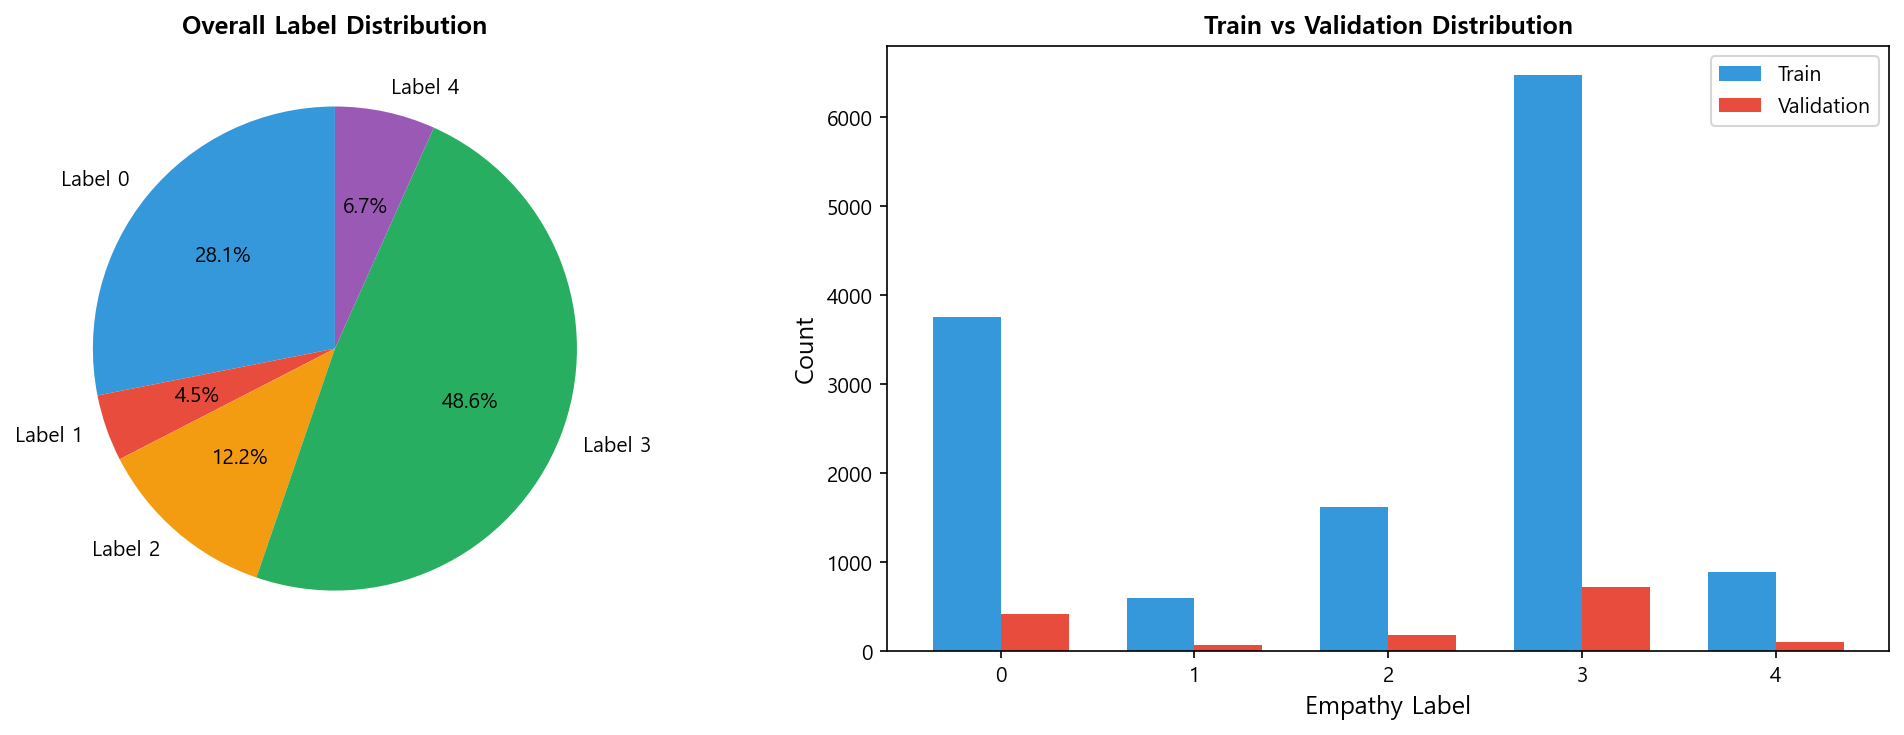
\includegraphics[width=0.95\textwidth]{figures/label_distribution.png}
    \caption{Empathy Label Distribution}
    
    \vspace{0.5em}
    \footnotesize\textit{Note.} Left: Overall dataset distribution. Right: Train vs Validation distribution comparison.
\end{figure}

\subsection{Train/Validation Split}

\begin{table}[H]
\centering
\caption{Train and Validation Set Label Distribution}
\label{tab:train_val}
\begin{tabular}{lrrrr}
\toprule
\textbf{Label} & \textbf{Train} & \textbf{Train \%} & \textbf{Val} & \textbf{Val \%} \\
\midrule
0 & 3,750 & 28.1\% & 417 & 28.1\% \\
1 & 594 & 4.5\% & 66 & 4.4\% \\
2 & 1,625 & 12.2\% & 181 & 12.2\% \\
3 & 6,478 & 48.6\% & 720 & 48.5\% \\
4 & 894 & 6.7\% & 100 & 6.7\% \\
\midrule
\textbf{Total} & \textbf{13,341} & \textbf{100\%} & \textbf{1,484} & \textbf{100\%} \\
\bottomrule
\end{tabular}

\vspace{0.5em}
\footnotesize\textit{Note.} Stratified sampling was used with a 90:10 split ratio.
\end{table}

% ============================================
% 3. Methodology
% ============================================
\section{Methodology}

\subsection{Model Configuration}

\begin{table}[H]
\centering
\caption{Model Configuration Comparison}
\label{tab:model_config}
\begin{tabular}{lll}
\toprule
\textbf{Parameter} & \textbf{GPT-4.1 Nano} & \textbf{DeepSeek 7B} \\
\midrule
Base Model & gpt-4.1-nano-2025-04-14 & DeepSeek-R1-Distill-Qwen-7B \\
Parameters & Unknown (API) & 7 Billion \\
Training Method & Supervised Fine-tuning & QLoRA (4-bit + LoRA) \\
Platform & OpenAI API & Google Colab (H100) \\
Quantization & N/A & 4-bit NF4 \\
LoRA Rank & N/A & 16 \\
Learning Rate & Auto & 2e-4 \\
Batch Size & Auto & 16 (effective) \\
Epochs & 3 & 3 \\
Training Time & $\sim$30 min & $\sim$3 hours \\
\bottomrule
\end{tabular}

\vspace{0.5em}
\footnotesize\textit{Note.} GPT fine-tuning via OpenAI API; DeepSeek via QLoRA on Colab.
\end{table}

\subsection{QLoRA Methodology}

QLoRA (Quantized Low-Rank Adaptation) enables efficient fine-tuning of large models:

\begin{enumerate}
    \item \textbf{4-bit Quantization}: Reduces model weights to 4-bit precision (NF4)
    \item \textbf{LoRA Adapters}: Trains only 0.5\% of parameters while freezing the rest
    \item \textbf{Double Quantization}: Further reduces memory by quantizing quantization constants
\end{enumerate}

\begin{figure}[H]
    \centering
    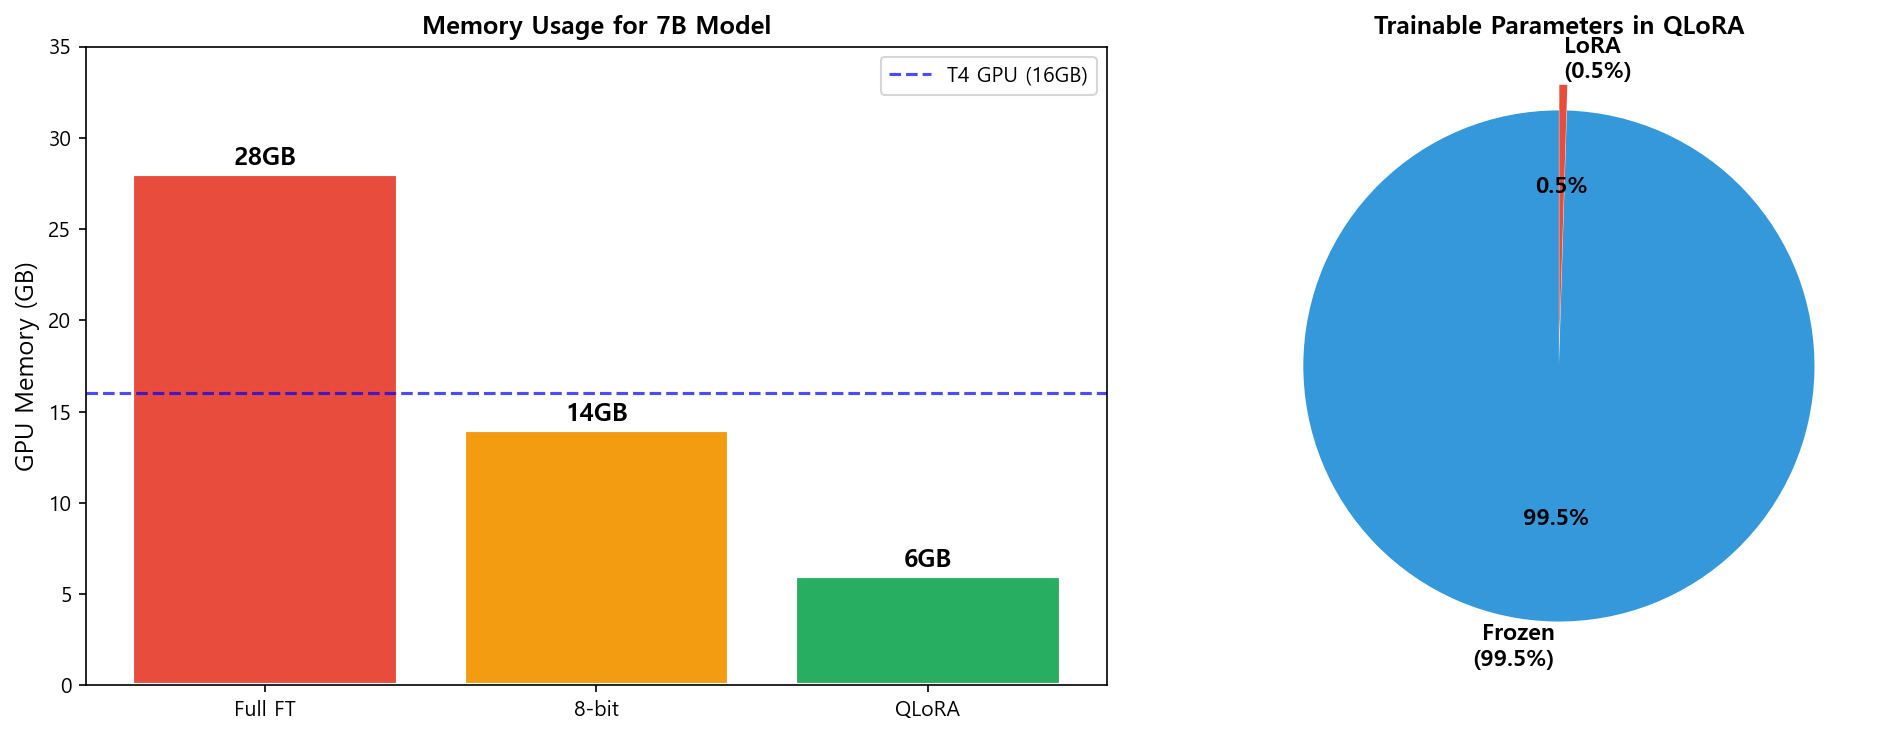
\includegraphics[width=0.95\textwidth]{figures/qlora_explanation.png}
    \caption{QLoRA Memory Efficiency}
    
    \vspace{0.5em}
    \footnotesize\textit{Note.} Left: GPU memory comparison for 7B model. Right: Trainable parameter ratio in QLoRA.
\end{figure}

\subsection{Prompt Design}

The prompt structure used for model training and inference:

\begin{verbatim}
[System] You are an empathy classifier for Korean persona-user 
dialogues. Output JSON with "empathy_label" (0-4).

[User] Classify the empathy level of the PERSONA's reply.
USER: [user utterance]
PERSONA: [persona response]
Return JSON only.
\end{verbatim}

% ============================================
% 4. Experimental Results
% ============================================
\section{Experimental Results}

\subsection{Overall Performance Comparison}

\begin{table}[H]
\centering
\caption{Overall Model Performance Comparison}
\label{tab:overall_results}
\begin{tabular}{lccccc}
\toprule
\textbf{Metric} & \textbf{GPT Base} & \textbf{GPT FT} & \textbf{DeepSeek} & \textbf{Best Impr.} \\
\midrule
Accuracy & 15.70\% & 33.49\% & \textbf{49.19\%} & +33.49\%p \\
Macro Precision & 0.2272 & 0.2270 & 0.3067 & +0.0795 \\
Macro Recall & 0.1939 & 0.2326 & 0.2284 & +0.0345 \\
Macro F1 & 0.1452 & \textbf{0.2275} & 0.2034 & +0.0823 \\
Correct / Total & 233/1484 & 497/1484 & \textbf{730/1484} & +497 \\
\bottomrule
\end{tabular}

\vspace{0.5em}
\footnotesize\textit{Note.} DeepSeek achieved highest accuracy (49.19\%); GPT FT achieved highest Macro F1 (0.2275).
\end{table}

\begin{figure}[H]
    \centering
    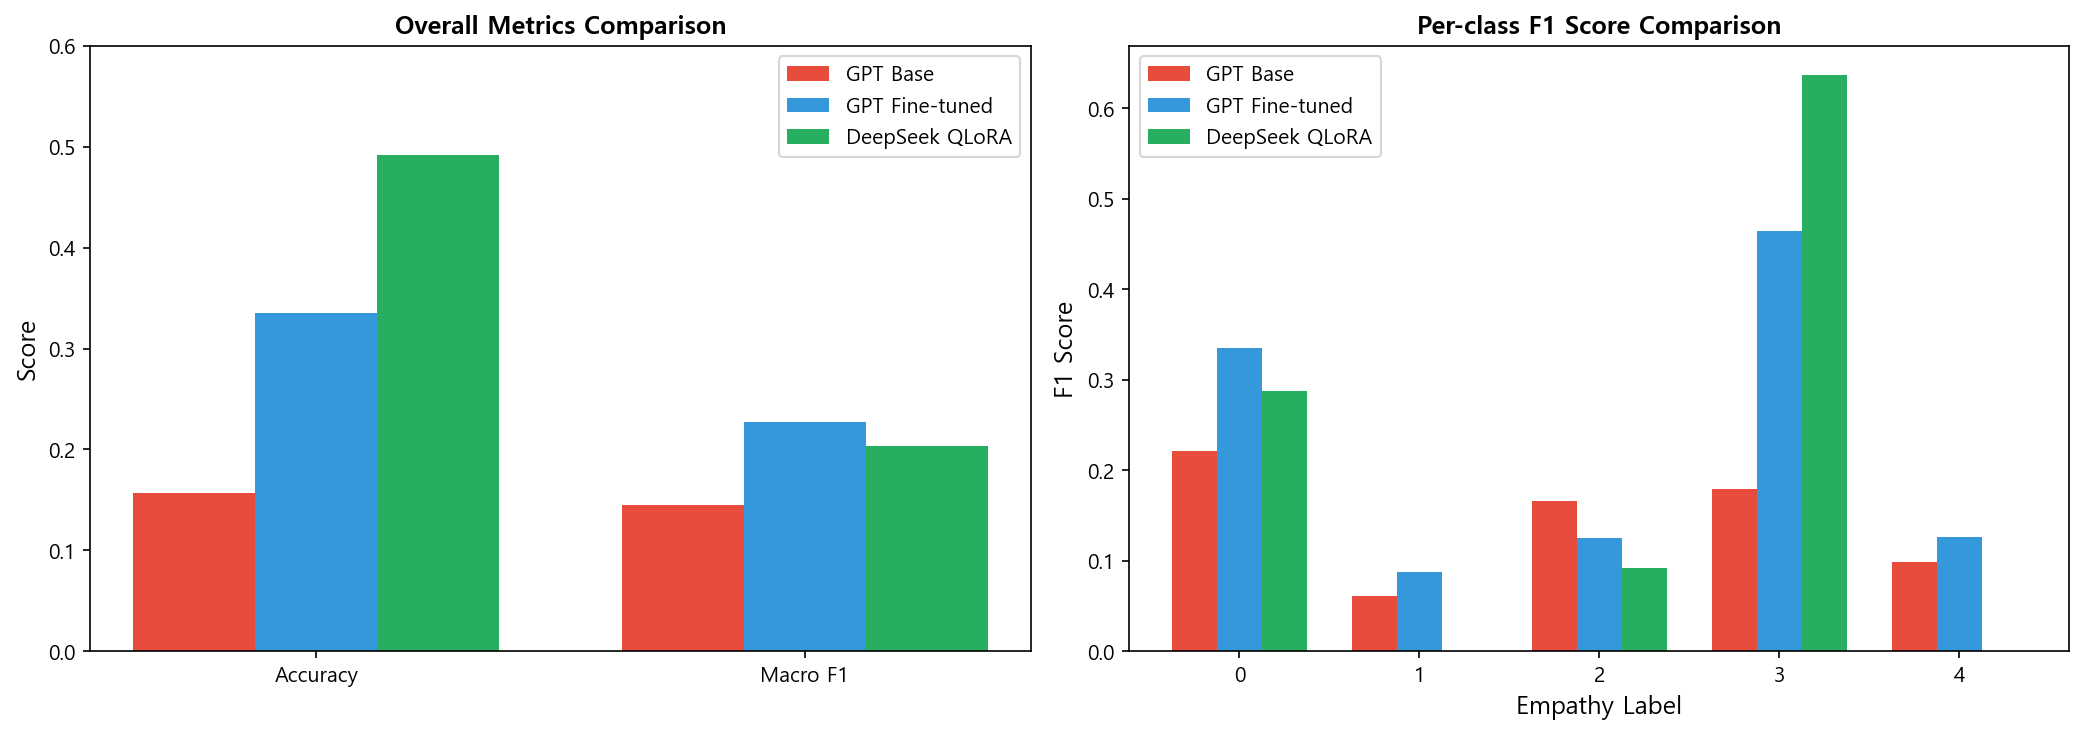
\includegraphics[width=0.95\textwidth]{figures/model_comparison.png}
    \caption{Model Performance Comparison}
    
    \vspace{0.5em}
    \footnotesize\textit{Note.} Left: Overall metrics comparison. Right: Per-class F1 score comparison.
\end{figure}

\begin{figure}[H]
    \centering
    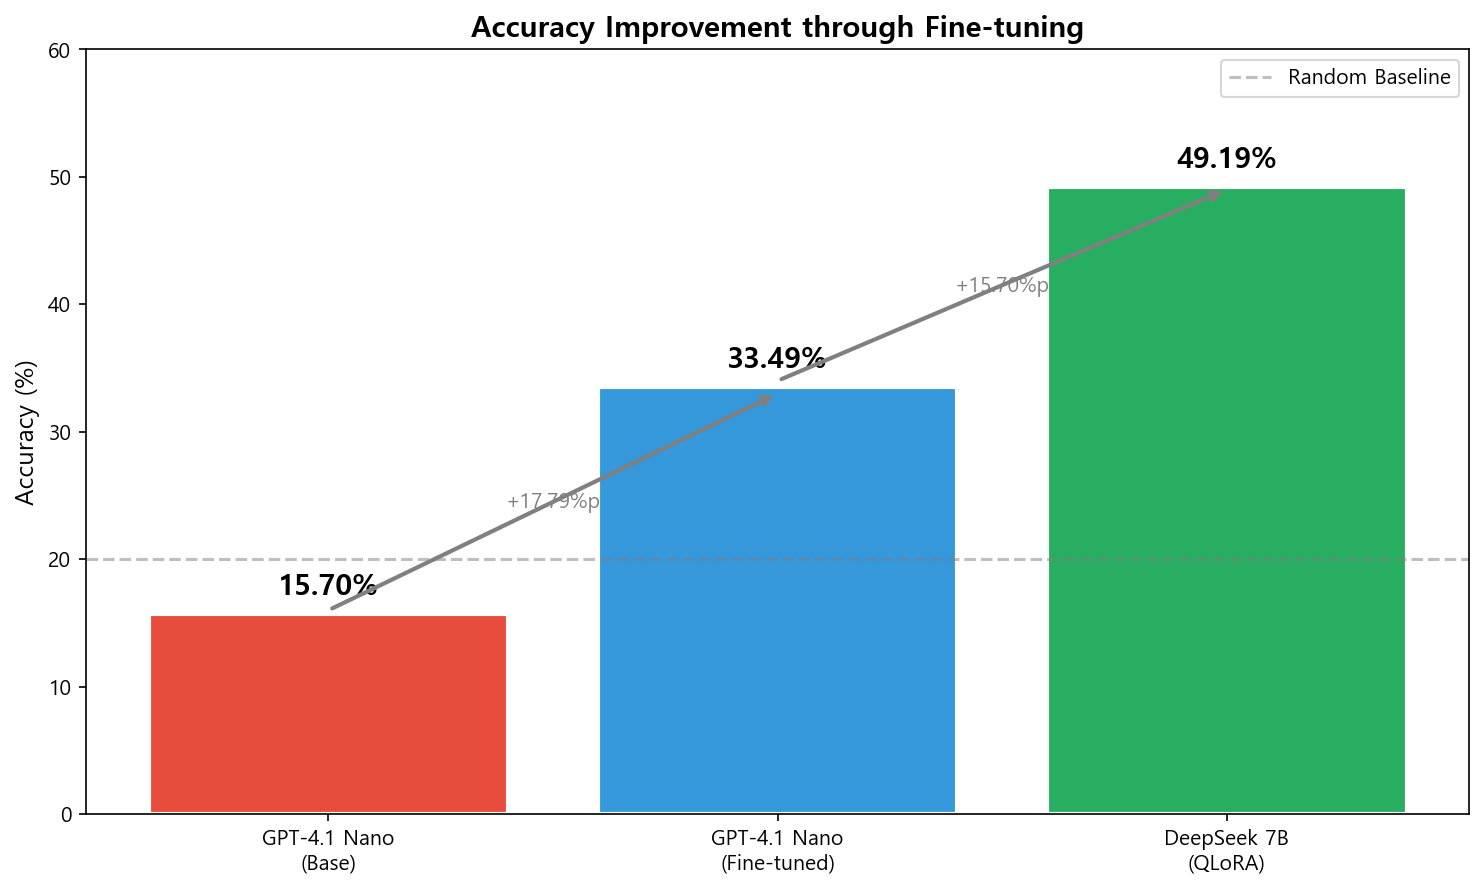
\includegraphics[width=0.7\textwidth]{figures/accuracy_improvement.png}
    \caption{Accuracy Improvement through Fine-tuning}
    
    \vspace{0.5em}
    \footnotesize\textit{Note.} DeepSeek QLoRA achieved +33.49\%p improvement over base model.
\end{figure}

\subsection{Per-Class Performance Analysis}

\begin{table}[H]
\centering
\caption{Per-Class Performance Metrics}
\label{tab:per_class}
\begin{tabular}{l|ccc|ccc|ccc}
\toprule
 & \multicolumn{3}{c|}{\textbf{GPT Base}} & \multicolumn{3}{c|}{\textbf{GPT FT}} & \multicolumn{3}{c}{\textbf{DeepSeek}} \\
\textbf{Label} & P & R & F1 & P & R & F1 & P & R & F1 \\
\midrule
0 & .431 & .149 & .221 & .339 & .331 & .335 & .433 & .216 & .288 \\
1 & .036 & .227 & .061 & .074 & .106 & .087 & .000 & .000 & .000 \\
2 & .108 & .354 & .166 & .118 & .133 & .125 & .600 & .050 & .092 \\
3 & .482 & .110 & .179 & .500 & .433 & .464 & .501 & .876 & \textbf{.637} \\
4 & .080 & .130 & .099 & .104 & .160 & .126 & .000 & .000 & .000 \\
\bottomrule
\end{tabular}

\vspace{0.5em}
\footnotesize\textit{Note.} P = Precision, R = Recall. DeepSeek excels at Label 3 (F1=0.637) but fails on Labels 1, 4.
\end{table}

\subsection{Confusion Matrix Analysis}

\begin{figure}[H]
    \centering
    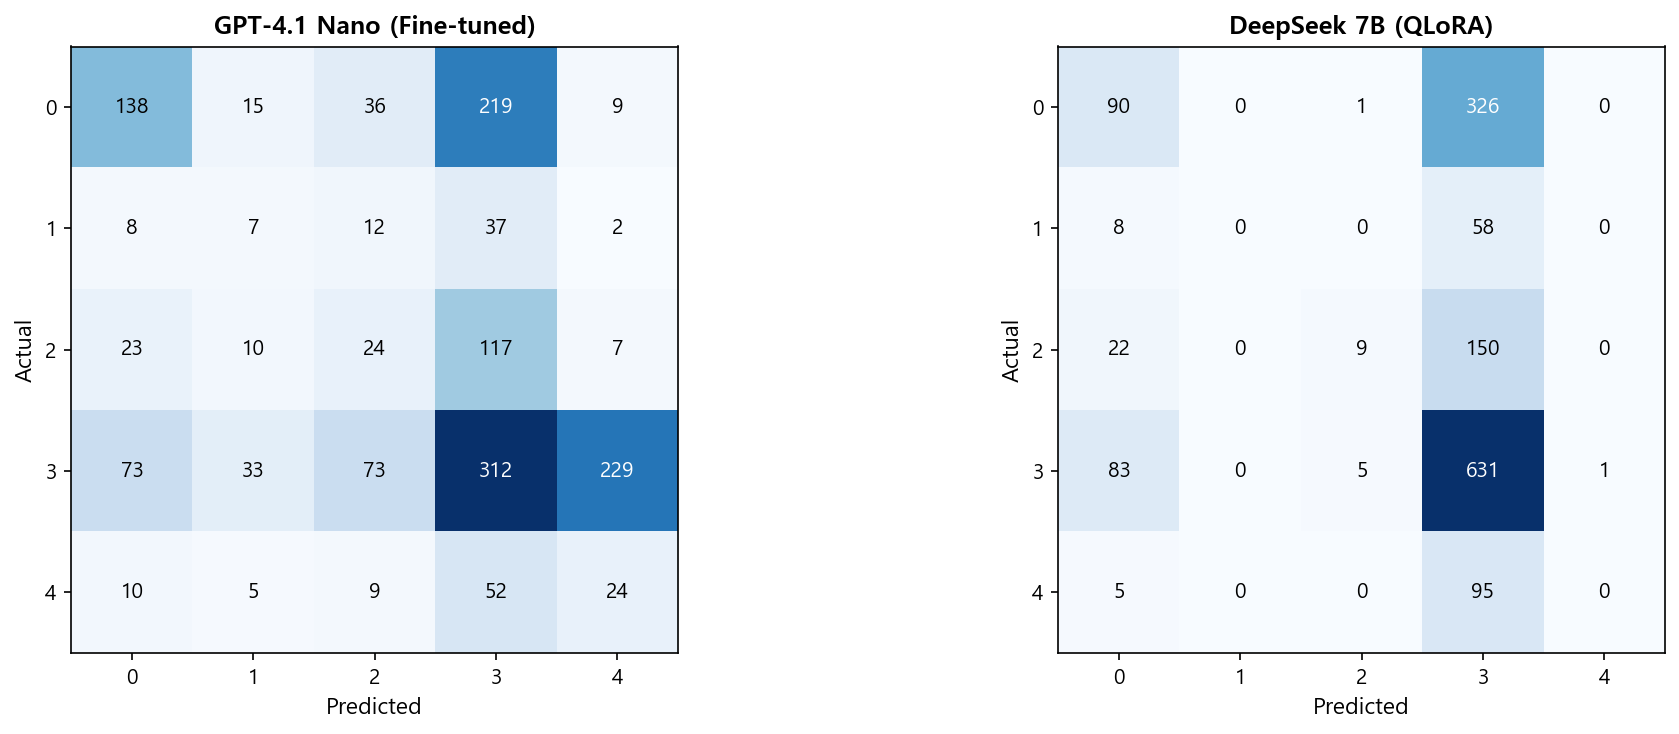
\includegraphics[width=0.95\textwidth]{figures/confusion_matrix.png}
    \caption{Confusion Matrices for Fine-tuned Models}
    
    \vspace{0.5em}
    \footnotesize\textit{Note.} Left: GPT Fine-tuned. Right: DeepSeek QLoRA. DeepSeek shows strong bias toward Label 3.
\end{figure}

\begin{table}[H]
\centering
\caption{DeepSeek Confusion Matrix}
\label{tab:ds_cm}
\begin{tabular}{l|ccccc|c}
\toprule
 & \multicolumn{5}{c|}{\textbf{Predicted}} & \\
\textbf{Actual} & 0 & 1 & 2 & 3 & 4 & \textbf{Total} \\
\midrule
0 & \textbf{90} & 0 & 1 & 326 & 0 & 417 \\
1 & 8 & \textbf{0} & 0 & 58 & 0 & 66 \\
2 & 22 & 0 & \textbf{9} & 150 & 0 & 181 \\
3 & 83 & 0 & 5 & \textbf{631} & 1 & 720 \\
4 & 5 & 0 & 0 & 95 & \textbf{0} & 100 \\
\midrule
\textbf{Total} & 208 & 0 & 15 & 1260 & 1 & 1484 \\
\bottomrule
\end{tabular}

\vspace{0.5em}
\footnotesize\textit{Note.} Bold values indicate correct predictions. 84.9\% of predictions are Label 3.
\end{table}

% ============================================
% 5. Text Analysis
% ============================================
\section{Text Analysis}

\subsection{Text Length Distribution}

\begin{figure}[H]
    \centering
    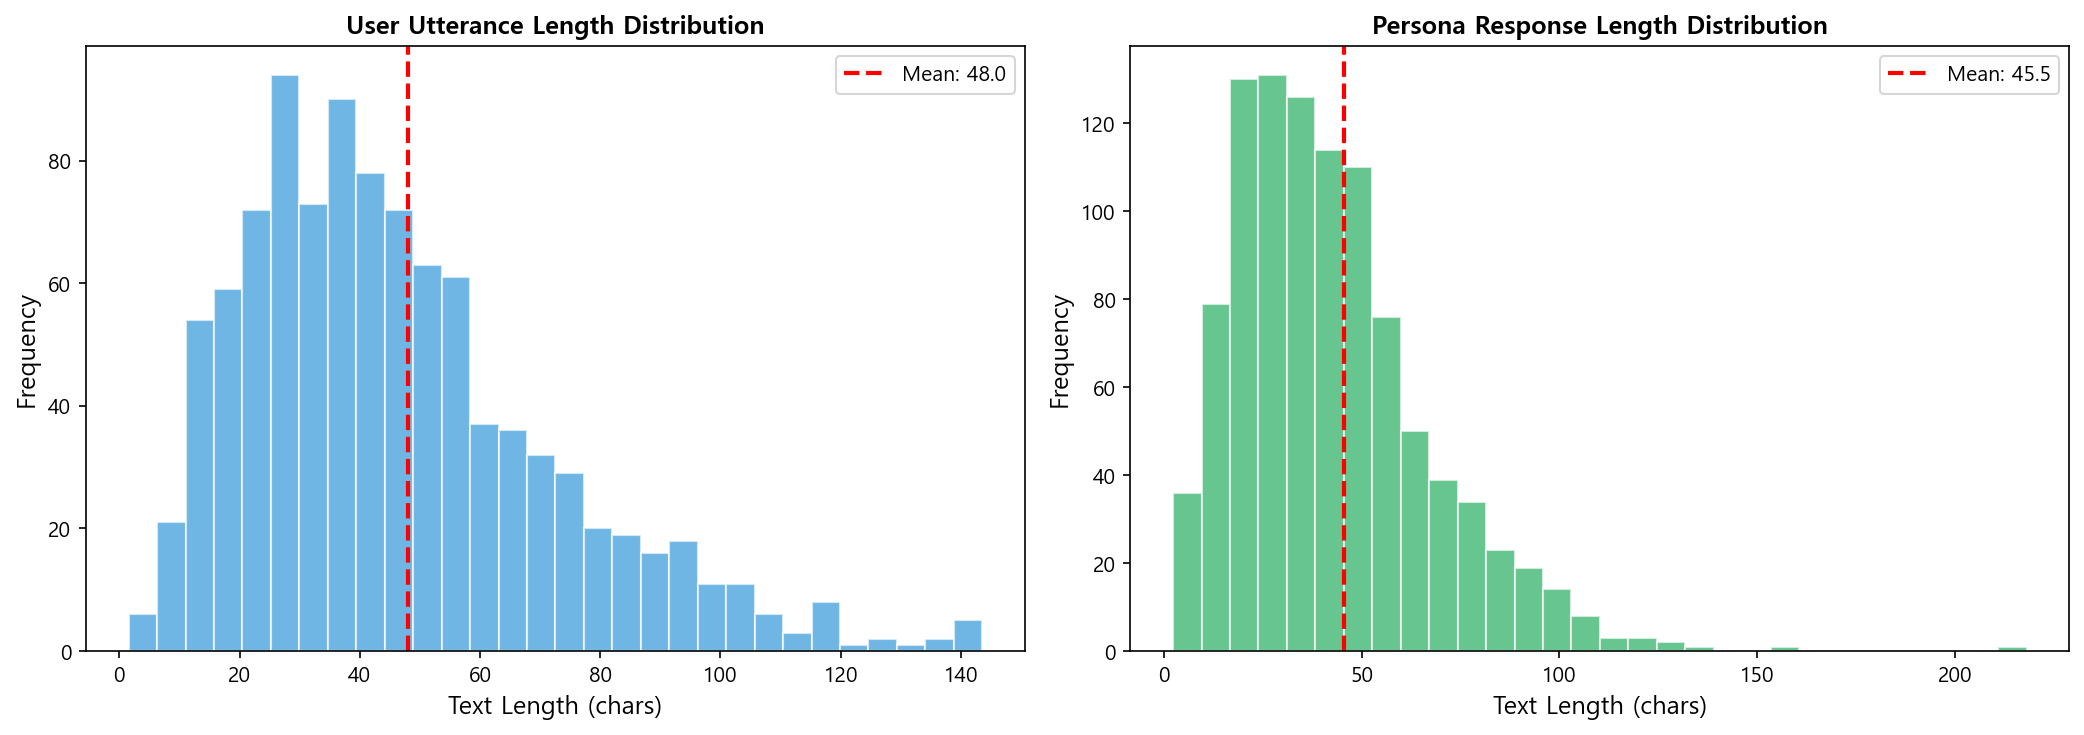
\includegraphics[width=0.95\textwidth]{figures/text_length.png}
    \caption{Text Length Distribution}
    
    \vspace{0.5em}
    \footnotesize\textit{Note.} Left: User utterance length. Right: Persona response length. Red dashed line indicates mean.
\end{figure}

\subsection{Response Length by Empathy Level}

\begin{figure}[H]
    \centering
    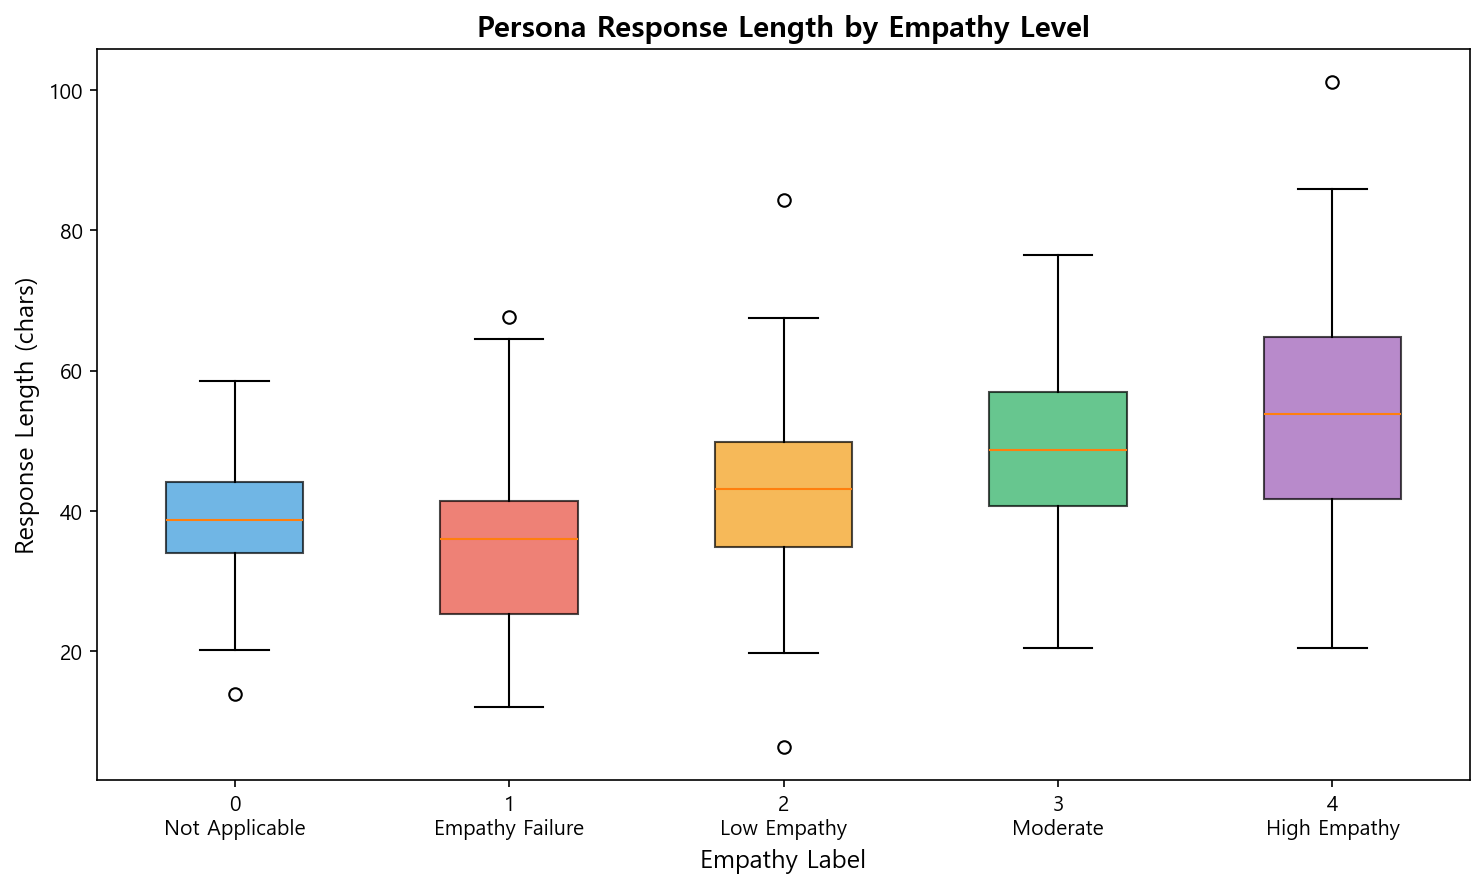
\includegraphics[width=0.7\textwidth]{figures/response_length_by_label.png}
    \caption{Persona Response Length by Empathy Level}
    
    \vspace{0.5em}
    \footnotesize\textit{Note.} Higher empathy levels tend to have longer responses.
\end{figure}

\subsection{Model Behavior Analysis}

Key observations from the experimental results:

\begin{enumerate}
    \item \textbf{DeepSeek's Label 3 Bias}: DeepSeek predicts Label 3 for 84.9\% of samples, leading to high accuracy on the majority class but zero performance on Labels 1 and 4.
    
    \item \textbf{GPT's Balanced Predictions}: GPT Fine-tuned shows more balanced predictions across all classes, resulting in higher Macro F1 despite lower overall accuracy.
    
    \item \textbf{Class Imbalance Impact}: Both models struggle with minority classes (Labels 1, 4), which comprise only 4.5\% and 6.7\% of the data respectively.
\end{enumerate}

% ============================================
% 6. Conclusion
% ============================================
\section{Conclusion}

\subsection{Key Achievements}

This project developed a system that automatically classifies empathy levels in Korean conversations using the OPELA dataset. Key achievements include:

\begin{itemize}
    \item Built empathy classification model using OPELA dataset (14,825 samples)
    \item GPT-4.1 Nano fine-tuning: 15.70\% $\rightarrow$ 33.49\% (+17.79\%p)
    \item DeepSeek 7B QLoRA fine-tuning: 15.70\% $\rightarrow$ \textbf{49.19\%} (+33.49\%p)
    \item Demonstrated QLoRA efficiency: 7B model trained on free Colab GPU
    \item Identified trade-off between accuracy and class balance
\end{itemize}

\subsection{Model Comparison Summary}

\begin{table}[H]
\centering
\caption{Final Model Comparison}
\label{tab:final_comparison}
\begin{tabular}{lcc}
\toprule
\textbf{Aspect} & \textbf{GPT-4.1 Nano FT} & \textbf{DeepSeek QLoRA} \\
\midrule
Accuracy & 33.49\% & \textbf{49.19\%} \\
Macro F1 & \textbf{0.2275} & 0.2034 \\
Minority Class Handling & Better & Poor \\
Training Cost & API credits & Free (Colab) \\
Reproducibility & Limited & Full \\
\bottomrule
\end{tabular}

\vspace{0.5em}
\footnotesize\textit{Note.} Choice depends on priority: accuracy (DeepSeek) vs. class balance (GPT).
\end{table}

\subsection{Limitations and Future Work}

\textbf{Limitations:}
\begin{itemize}
    \item Severe class imbalance (Label 3 = 48.6\% of data)
    \item DeepSeek ignores minority classes (Labels 1, 4)
    \item 5-class classification may be too fine-grained for the task
\end{itemize}

\textbf{Future Work:}
\begin{enumerate}
    \item Class simplification: 5-class $\rightarrow$ 3-class (Low/Medium/High)
    \item Data augmentation for minority classes
    \item Ensemble of GPT and DeepSeek models
    \item LLaMA 3.1 8B fine-tuning for comparison
    \item Class-weighted loss function for balanced training
\end{enumerate}

% ============================================
% References
% ============================================
\section*{References}
\addcontentsline{toc}{section}{References}

Smilegate AI \& Seoul National University (2022). OPELA: Open-domain conversations by Personas with Empathy, Long-term memory, and Attractive personality. GitHub: \url{https://github.com/smilegate-ai/OPELA}

Lee, Y. K., Cho, W. I., Bae, S., Choi, H., Park, J., Kim, N. S., \& Hahn, S. (2022). ``Feels like I've known you forever'': empathy and self-awareness in human open-domain dialogs. PsyArXiv.

Dettmers, T., Pagnoni, A., Holtzman, A., \& Zettlemoyer, L. (2023). QLoRA: Efficient Finetuning of Quantized LLMs. NeurIPS.

Hu, E. J., Shen, Y., Wallis, P., Allen-Zhu, Z., Li, Y., Wang, S., \& Chen, W. (2021). LoRA: Low-Rank Adaptation of Large Language Models. ICLR.

DeepSeek AI (2024). DeepSeek-R1: Advancing Reasoning in Large Language Models.

\end{document}
